\section{Ordinary Least Squares (OLS)}
\subsection{Theory} \todo{}

\subsection{Assumptions} \todo{add here}
\begin{itemize}
	\item Very sensitive to outliers (need outliers rejection eg. RANSAC)
	\item System must be linear
	\item Residual error only in dependent variable
	\item Test the significance of the model using an extra sum of squares test on the R$^2$ value
\end{itemize}
\subsection{Equations}
\[
AX=L+V 
\]
\[
m = \text{number of observations} \hspace{1cm} 
n = \text{number of unknowns}
\]
\[
dof = \text{degrees of freedom (\# of redundant observations)} = m-n
\]
\[
A = \begin{bmatrix}
a_{11} & a_{12} & \dots & a_{1n} \\
a_{21} & a_{22} & \dots & a_{1n} \\
\vdots & \vdots & \vdots& \vdots \\
a_{m1} & a_{m2} & \dots & a_{mn} \\
\end{bmatrix}
\hspace{1cm}
X = 
\begin{bmatrix}
x_1 \\ x_2 \\ \vdots \\ x_n
\end{bmatrix}
\hspace{1cm}
L = 
\begin{bmatrix}
l_1 \\ l_2 \\ \vdots \\ l_m
\end{bmatrix}
\hspace{1cm}
V = 
\begin{bmatrix}
v_1 \\ v_2 \\ \vdots \\ v_m
\end{bmatrix}
\]
\begin{align*}
\text{Unknowns} &= \hat{X} = inv(A^TA)A^TL\\
\text{Residuals} &= V = AX - L\\
\text{Reference Variance} &= S_0^2 = \dfrac{V'V}{dof} \\
\text{Cofactor Matrix} &= Q = inv(A^TA) \\
\text{Covariance Matrix} &= \Sigma = S_0^2 \times Q \\
\text{Standard Deviation of Solved Unknowns} &= \sigma_{\hat{X}} = \sqrt{diag(\Sigma)} \\
\text{Predicted L} &= \hat{L} = AX \\
\text{R$^2$ (model skill)} &= \dfrac{var(\hat{L})}{var(L)} \\
\text{RMSE } &= \sqrt{\dfrac{V^2}{m}} \\
\end{align*}
\clearpage
\subsection{Sample Problem}
Given the Points: 
\[
x = [0,1,2,3,4] \hspace{1cm} y = [0,1,7,13,24]
\]
Fit a parabola given the observation equation:
\[
y = a x^2 +b x + c
\]
Note that the observation equation is linear. The x$^2$ term is a constant once observation values are substituted.
\[
A = \begin{bmatrix}
x_1^2 & x_1 & 1 \\
x_2^2 & x_2 & 1 \\
x_3^2 & x_3 & 1 \\
x_4^2 & x_4 & 1 \\
x_5^2 & x_5 & 1 \\
\end{bmatrix} =
\begin{bmatrix}
0 & 0 & 1 \\
1 & 1 & 1 \\
4 & 2 & 1 \\
9 & 3 & 1 \\
16 & 4 & 1 \\
\end{bmatrix}
\hspace{1cm}
X = 
\begin{bmatrix}
a \\ b \\ c 
\end{bmatrix}
\hspace{1cm}
L =
\begin{bmatrix}
y_1 \\ y_2 \\ y_3 \\ y_4 \\ y_5
\end{bmatrix} = 
\begin{bmatrix}
0 \\ 1 \\ 7 \\ 13 \\ 24
\end{bmatrix}
\]
Use the Equations and solve:
\begin{table}[htbp]
	\centering
	\begin{tabular}{|c|c|c|}
		\toprule
		$dof = 2$
		&
		$\hat{X} = 
		\begin{bmatrix}
		1.43\\0.29\\-0.14
		\end{bmatrix}$
		&
		$V = 
		\begin{bmatrix}
		-0.14\\0.57\\-0.86\\0.57\\-0.14
		\end{bmatrix}$
		\\	\midrule
		$Q = \begin{bmatrix}
		0.07 & -0.29 & 0.14 \\ 
		-0.29 & 1.24 & -0.77 \\ 
		0.14 & -0.77 & 0.89 \\ 
		\end{bmatrix}$
		&
		$S_0^2 = 0.71$
		&
		$\hat{L} = 
		\begin{bmatrix}
		-0.14\\1.57\\6.14\\13.57\\23.86
		\end{bmatrix}$
		\\	\midrule
		$\Sigma_{\hat{X}} = \begin{bmatrix}
		0.05 & -0.20 & 0.10 \\ 
		-0.20 & 0.89 & -0.55 \\ 
		0.10 & -0.55 & 0.63 \\ 
		\end{bmatrix}$
		&
		$\sigma_{\hat{X}} = 
		\begin{bmatrix}
		0.05\\0.89\\0.63 
		\end{bmatrix}$
		&
		$R^2 = 0.9963$
		\\
		\bottomrule
	\end{tabular}%
\end{table}%
\begin{figure}[H]
	\centering
	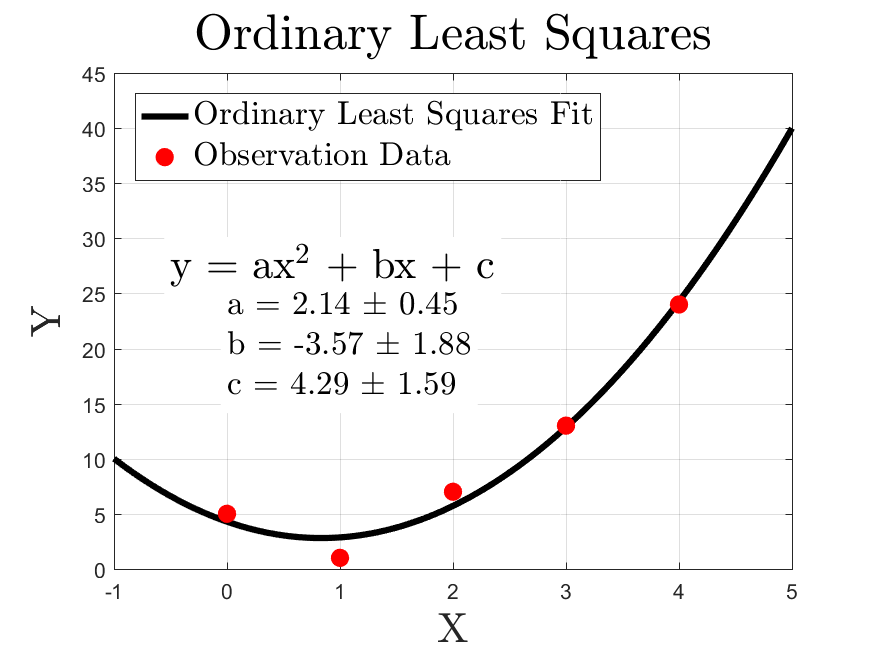
\includegraphics[height = 3.5in]{OLSexample.png}
\end{figure}
\clearpage

\subsection{Example Matlab Code}
\lstinputlisting[
label      = {alg:exampleOLS},
caption    = {exampleOLS.m},
style      = Matlab-editor,
basicstyle = \mlttfamily,
firstline  = 1,
lastline   = 17,
firstnumber= 1
]{exampleOLS.m}

\lstinputlisting[
label      = {alg:exampleOLSplot},
caption    = {exampleOLS.m (plotting Code)},
style      = Matlab-editor,
basicstyle = \mlttfamily,
firstline  = 19,
lastline   = 45,
firstnumber= 19
]{exampleOLS.m}